\graphicspath{{./images/}}      
\def\CHAPTERONE{./chapters/Chapter-1} 

\chapter{Experimente}
\label{chap:experiments}
%	\input{\CHAPTERONE /motivation}

Im folgenden Kapitel werden die Experimente beschrieben, die im Rahmen dieser Arbeit durchgeführt wurden, um die Objekterkennung in fotorealistischen Bildern zu evaluieren. Für die Experimente wurden mit dem in Kapitel \ref{sec:takingpics} vorgestellten Verfahren 114 Szenen erstellt und von ihnen fünf Bilder aufgenommen. Jedes Objekt ist einem oder mehreren folgender Szenarios zugeordnet: \textit{breakfast}, \textit{cooking} oder \textit{fridge}. Die Zuordnung ist in Tabelle \ref{tab:objects} einzusehen. Eine Szene enthält nur Objekte eines Szenarios. Dies ist echten Bedingungen nachempfunden, denn in der Regel finden sich im Kühlschrank keine Gabeln, Milch allerdings schon, sowie auch auf einem Frühstückstisch. Es wurden so 50 \textit{breakfast} und \textit{cooking} Szenen und 14 \textit{fridge} Szene erstellt. Insgesamt stehen so 570 Unreal-Bilder zur Verfügung. \par
In einem ersten Experiment wird ein Klassifizierer trainiert und mit den Unreal-Bildern getestet. \todo{ausweiten?} 


\section{Klassifizierung über Merkmale}
\label{sec:classificationExperiment}
Die zuvor erstellten Unreal-Bilder werden in einem ersten Experiment über Merkmale klassifiziert. Dazu wird ein Annotator aus dem \robosherlock-Paket \textit{rs\_addons} als Klassifizierer mit echten Bildern der verwendeten Objekte trainiert. Mehr zu dem Paket und den Klassifizieren ist in \ref{sec:classifiers} auf Seite \pageref{sec:classifiers} zu finden. \par

Als Klassifizierer wird der RFAnnotator benutzt, der auf einer \textit{Random-Forest} Implementierung basiert. Die zu unterscheidenden 20 Klassen sind in der Tabelle \ref{tab:objects} zu finden. Diese Bilder der echten Objekte wurden den Klassen zugeordnet, bevor der Klassifizierer damit trainiert wurde. Da es sich um einen Annotator für \robosherlock handelt, wurde eine \gls{ae} mit einigen \textit{hyotheses generators}, dem CaffeAnnotator zum Extrahieren der Merkmale (siehe Kap. \ref{sec:caffeAnno}, S.\pageref{sec:caffeAnno}), dem UnrealGTAnnotator zum herausziehen der \gls{gt} aus den Unreal-Bildern und dem Klassifizierer erstellt. Um die Ergebnisse später verarbeiten zu können werden sie mit dem MLNInference (siehe Kap. \ref{sec:mlnInferencer}, S. \pageref{sec:mlnInferencer}) als logische Prädikate ausgegeben. \par
 
Die so erhaltene Klassifizierung für jedes Objekt wird mit der \gls{gt} verglichen, um so die Erkennungsrate des Klassifizierers zu ermitteln. Die Ergebnisse sind in Figur \ref{fig:classi_Ex_confMatrix} und Tabelle \ref{tab:classi_Ex_classMetrics} abgebildet. Während nahezu alle Objekte eine \gls{accuracy} über 90\% aufweisen, zeigen \gls{precision}, \gls{recall} und gls{f1score}, dass der RFAnnoator große Schwierigkeiten hat, ähnliche Objekte auseinander zu halten. Besonders häufig werden Objekte fälschlicherweise als Milch(Milk) und Salz(TableSalt)  eingeordnet. Dies ist auf box-artige und Farbähnlichkeit vieler Objekte mit der Milch und dem Salz zurückzuführen, welche in insgesamt in größerer Zahl in den Daten vorkommen als andere Objektklassen. Des weiteren hat der Klassifizierer Schwierigkeiten das Geschirr auseinander zu halten, was auf die Größe dessen zurückzuführen ist. Besonders schlecht schneidet der Pfannenwender(Spatula) ab, der nicht einmal korrekt erkannt wurde. Mit einem \gls{f1score} über 0,8 schneiden die Objektklassen Buttermilch(Buttermilk), Kaffee(Coffee), Becher(Cup) und PancakeMix am besten ab. Diese Klassen unterscheiden sich in Form (Buttermilk, PancakeMix) und Farbe (Coffee, Cup) stark von den anderen Objekten.  

\begin{figure}
	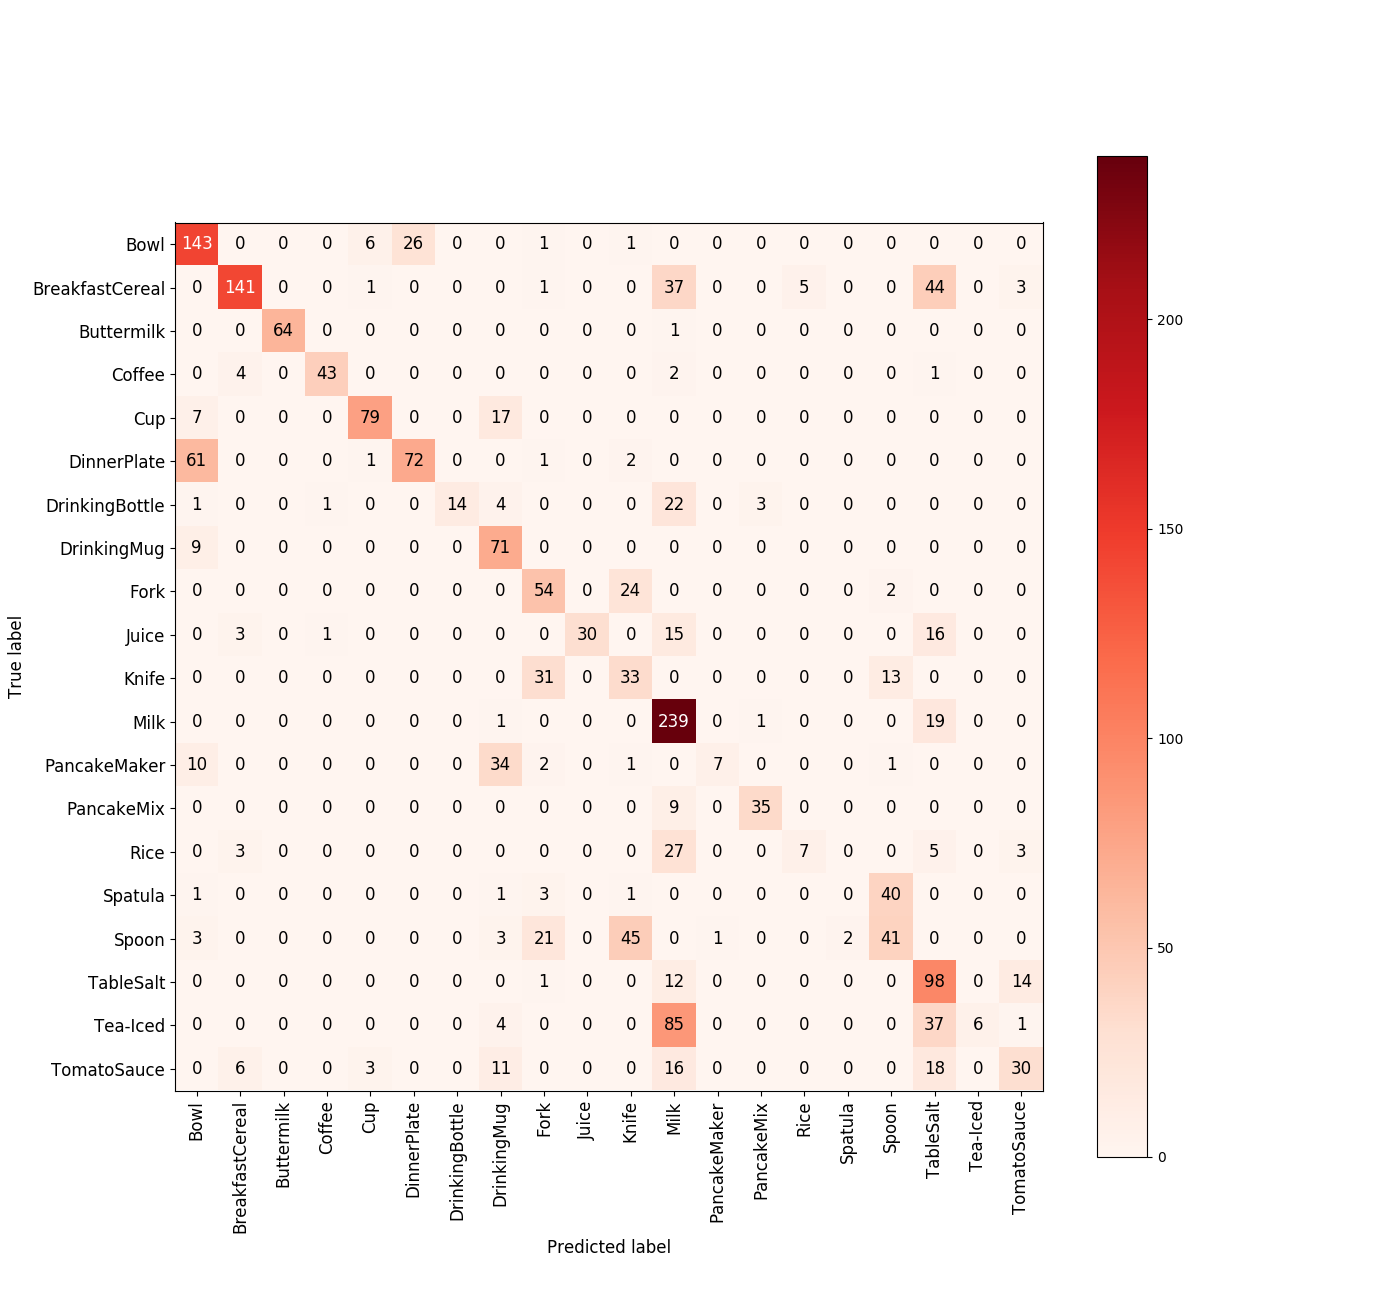
\includegraphics[scale=.5]{img/chapter6/classifierRFconf_matrix.png}
\caption[Ergebnisse der Klassifizierung durch den RFAnnotators]{Die Konfusionsmatrix für die Klassifikation der Unreal-Bilder durch den RFAnnotator.}
\label{fig:classi_Ex_confMatrix}
\end{figure}

\begin{table}
\rowcolors{1}{}{lightgray}
\begin{tabularx}{\textwidth}{Xllll}
\textbf{Objekt}	& \textbf{\gls{accuracy}} & \textbf{\gls{precision}}	& \textbf{\gls{recall}}	& \textbf{\gls{f1score}} \\ \hline
Bowl & 0.91 & 0.61 & 0.81 & 0.69 \\  
BreakfastCereal & 0.92 & 0.9 & 0.61 & 0.72 \\  
Buttermilk & 1.0 & 1.0 & 0.98 & 0.99 \\  
Coffee & 0.99 & 0.96 & 0.86 & 0.91 \\  
Cup & 0.97 & 0.88 & 0.77 & 0.82 \\  
DinnerPlate & 0.93 & 0.73 & 0.53 & 0.61 \\  
DrinkingBottle & 0.97 & 1.0 & 0.31 & 0.47 \\  
DrinkingMug & 0.93 & 0.49 & 0.89 & 0.63 \\  
Fork & 0.93 & 0.47 & 0.68 & 0.55 \\  
Juice & 0.97 & 1.0 & 0.46 & 0.63 \\  
Knife & 0.91 & 0.31 & 0.43 & 0.36 \\  
Milk & 0.83 & 0.51 & 0.92 & 0.66 \\  
PancakeMaker & 0.96 & 0.88 & 0.13 & 0.22 \\  
PancakeMix & 0.99 & 0.9 & 0.8 & 0.84 \\  
Rice & 0.97 & 0.58 & 0.16 & 0.25 \\  
Spatula & 0.96 & 0.0 & 0.0 & 0.0 \\  
Spoon & 0.9 & 0.42 & 0.35 & 0.38 \\  
TableSalt & 0.88 & 0.41 & 0.78 & 0.54 \\  
Tea-Iced & 0.9 & 1.0 & 0.05 & 0.09 \\  
TomatoSauce & 0.94 & 0.59 & 0.36 & 0.44 \\  
\end{tabularx}
\caption[Objekt spezifische Kenngrößen des RFAnnotators]{Kenngrößen für die einzelnen Objekte aus der Klassifizierung der Unreal-Bilder mit dem RFAnnotator.}
\label{tab:classi_Ex_classMetrics}
\end{table}

\section{Unreal-Bilder}
\label{sec:onlyUnrealImages}
In einem ersten Experiment werden nur Unreal-Bilder zum trainieren und testen des \gls{mln} benutzt. Die logischen Prädikate wurden dazu mit der in Kapitel \ref{sec:analysisengine} vorgestellten \gls{ae} aus den 570 Unreal-Bildern extrahiert. Diese werden wie in Tabelle \ref{tab:annotators} auf S.\pageref{tab:annotators} beschrieben für das Modell deklariert. Zusätzlich gibt es noch das $scene$-Prädikat und eine Einschränkung für das $object$-Prädikat:
\begin{itemize}
\item das $scene(scene)$ Prädikat ordnet die Szene in einen räumlichen Kontext ein. Die Domäne für das Prädikat ist $dom(scene) = \{breakfast, cooking, fridge\}$
\item das Prädikat $object$ wird folgendermaßen definiert: $object(cluster, object!)$. Der \glqq!\grqq \ Operator besagt, dass dieses Prädikat als funktionelle Einschränkung behandelt werden soll. Das bedeutet, dass immer exakt ein Atom wahr sein muss; alle anderen sind falsch.\footnote{\url{http://pracmln.org/mln_syntax.html}} Im Falle des obigen Prädikats bedeutet das, dass jedem Cluster genau eine Objektklasse zugeordnet sein muss. Dies macht im Rahmen des Modells Sinn, da ein Objekt nicht mehreren Klassen zugleich angehören kann und wurde auch von Nyga et al.\cite{pr2looking} in ihrer \gls{mln}-Deklaration angenommen.
\end{itemize}
Das Folgende \gls{mln} beschreibt die Zusammenhänge der einzelnen Informationen der Annotatoren und der Objektklassen:
\begin{align*}
& w_{1} \ shape(?c, +?sha) \wedge object(?c, +?obj) \\
& w_{2} \ color(?c, +?col) \wedge object(?c, +?obj) \\
& w_{3} \ size(?c, +?size) \wedge object(?c, +?obj) \\
& w_{4} \ instance(?c, +?inst) \wedge object(?c, +?obj) \\
& w_{5} \ goggles\_Logo(?c, +?comp) \wedge object(?c, +?obj)\\
& w_{6} \ goggles\_Text(?c, +?text) \wedge object(?c, +?obj)\\
& w_{7} \ goggles\_Product(?c, +?prod) \wedge object(?c, +?obj)\\
& w_{8} \ scene(+?s) \wedge object(?c, +?obj)\\
& w_{9} \ object(?c1, +?t1) \wedge object(?c2, +?t2) \wedge ?c1 =/= ?c2
\end{align*}
\textit{Hinweise zur Syntax von \pracmln:} Jeder Variable muss ein \glqq ?\grqq \ vorangestellt werden. Das \glqq +\grqq \ bedeutet, dass für jedes Element der Domäne dieser Variable eine Formel erstellt wird. \footnote{\url{http://pracmln.org/mln_syntax.html}}  \par
 
Ein \gls{mln} wurde mit \textit{Discriminative Pseudo-likelihood Learning with Custom Grounding}   trainiert. Es wurde die \textit{Discrimitive} Variante des Lernalgorithmus gewählt, da es ein genaueres Modell und geringeren Rechenaufwand bietet. Als Voraussetzung müssen bestimmte Prädikate bei den Anfragen entweder nur in den Anfragen oder der Evidenz vorkommen. Da in diesem Fall die Objektklasse erkannt werden soll, ist das $object$-Prädikat die einzige Anfrage and das trainierte \gls{mln}. In der Evidenz kommt es natürlich nicht vor, da die Objektklasse sonst schon bekannt wäre und nicht aus den anderen Eigenschaften darauf geschlossen werden muss. Die \textit{Custom Grounding} Variante bietet eine schnellere Rechenzeit, wenn die Formeln größtenteils aus Konjunktionen bestehen. Eine Regularisierung findet durch den Gaussian-Prior mit einem Mittelwert $\mu = 0$ und einer Standardabweichung $\sigma = 10$ statt. \par   
Um dieses Modell zu evaluieren wird 10-fache Kreuzvalidierung durchgeführt. Dies verhindert Überanpassung des Modells, also die Anpassung an die Trainingsdaten und damit einen Verlust der Generalität des Modells.

\begin{table}
\rowcolors{1}{}{lightgray}
\begin{tabularx}{\textwidth}{llccccc}
\textbf{Instanz}  				& \textbf{Klasse}	& \textbf{breakfast}	& \textbf{fridge}	& \textbf{cooking}	& \textbf{Unreal} & \textbf{Real} \\ \hline
AlbiHimbeerJuice				& Juice				& +			& +			& +			& 14	& 18	\\
BlueCeramicIkeaMug				& DrinkingMug		& +			& 			&			& 8		& 9\\
BlueMetalPlateWhiteSpeckles		& DinnerPlate		& 			& 			&	+		& 9		& 10\\
BluePlasticBowl					& Bowl				& +			& 			&			& 9		& 9\\
BluePlasticFork					& Fork				& 			& 			&	+		& 8		& 9\\
BluePlasticKnife				& Knife				& 			& 			&	+		& 8		& 9\\
BluePlasticSpoon				& Spoon				& +			& 			&			& 8		& 11\\
CupEcoOrange					& Cup				& +			& 			&	+		& 12	& 15\\
EdekaRedBowl					& Bowl				& +			& 			&			& 8		& 9\\
ElBrygCoffee					& Coffee			& +			& 			&			& 8		& 9\\
JaMilch							& Milk				& +			& +			&			& 13	& 14\\
JodSalz							& TableSalt			& 			& 			&	+		& 9		& 9\\
KelloggsCornFlakes				& BreakfastCereal	& +			& 			&			& 8		& 9\\
KelloggsToppasMini				& BreakfastCereal	& +			& 			&			& 8		& 9\\
KnusperSchokoKeks				& BreakfastCereal	& +			& 			&			& 8		& 8\\
KoellnMuesliKnusperHonigNuss	& BreakfastCereal	& +			& 			&			& 8		& 8	\\
LargeGreySpoon					& Spoon				& 			& 			&	+		& 9		& 8	\\
LinuxCup						& DrinkingMugin		& +			& 			&			& 8		& 0\\
LionCerealBox					& BreakfastCereal	& +			& 			&			& 8		& 9	\\
MarkenSalz						& TableSalt			& 			& 			&	+		& 9		& 8	\\
MeerSalz						& TableSalt			& 			& 			&	+		& 9		& 8	\\
MondaminPancakeMix				& PancakeMix		& 			& 			&	+		& 9		& 8	\\
NesquikCereal					& BreakfastCereal	& +			& 			&			& 8		& 9	\\
PfannerGruneIcetea				& Tea-Iced			& 			& +			&	+		& 13	& 14\\
PfannerPfirsichIcetea			& Tea-Iced			& 			& +			&	+		& 14	& 13\\
RedMetalBowlWhiteSpeckles		& Bowl				& +			& 			&			& 9		& 8\\
RedMetalCupWhiteSpeckles		& Cup				& +			& 			&			& 8		& 10\\
RedMetalPlateWhiteSpeckles		& DinnerPlate		& 			& 			&	+		& 9		& 9\\
RedPlasticFork					& Fork				& 			& 			&	+		& 8		& 9\\
RedPlasticKnife					& Knife				& 			& 			&	+		& 8		& 9\\
RedPlasticSpoon					& Spoon				& +			& 			&			& 9		& 10\\
ReineButterMilch				& Buttermilk		& +			& +			&			& 13	& 14\\
SeverinPancakeMaker				& PancakeMaker		& 			& 			&	+		& 10	& 10\\
SiggBottle						& DrinkingBottle	& 			& 			&	+		& 9		& 9\\
SlottedSpatula					& Spatula			& 			& 			&	+		& 9		& 8\\
SojaMilch						& Milk				& +			& +			&			& 13	& 14\\
SpitzenReis						& Rice				& 			& 			&	+		& 9		& 9\\
TomatoAlGustoBasilikum			& TomatoSauce		& 			& 			&	+		& 8		& 8\\
TomatoSauceOroDiParma			& TomatoSauce		& 			& 			&	+		& 9		& 8\\
VollMilch						& Milk				& +			& +			&			& 13	& 14\\
WeideMilchSmall					& Milk				& +			& +			&			& 13	& 14\\
WhiteCeramicIkeaBowl			& Bowl				& +			& 			&			& 8		& 9\\
YellowCeramicPlate				& DinnerPlate 	    & 			& 			&	+		& 9		& 6\\ \hline
\textbf{Insgesamt: 43}				& \textbf{20}		& \textbf{23} & \textbf{8} & \textbf{22} & & \\
\end{tabularx}
\caption[Objekte und ihre Verteilung in den Szenen]{Die Tabelle enthält alle Objekte und welchen Klassen sie zugeordnet sind, sowie die Zuordnung zu den Szenarien und wie häufig sie insgesamt in den Szenen vorkommen.}
\label{tab:objects}
\end{table}


\section{Echte Bilder}
  
Leider sind LinuxCup und YellowPlate nicht mehr zur Hand. Plate mit weißer Platte ersetzt. Cup fehlt.